\newpage
\chapter{Desenvolvimento}
\label{ch:desenvolvimento}

\par Este capítulo apresenta os passos de desenvolvimento dos recursos assistivos consolidados em uma biblioteca nomeada ICan.js.

\section{Arquitetura da biblioteca}

% (17/03/2019) -> Inserir nesta seção a arquitetura expandida da biblioteca, ou seja, todos os módulos disponíveis nela, isto facilita o entendimento (Esta ideia vem de parte da explicação realizada pelo Mineda).

\par Para iniciar o desenvolvimento da biblioteca, fez-se inicialmente a definição de sua arquitetura, em que esta foi separada em conjuntos de funcionalidades, como descrito em \cite{tensorflowjs2019}. Neste caso, os conjuntos são nomeados \textitbf{Core} e \textitbf{Common} e são construídos sobre as funções disponibilizadas pelo Tensorflow.js, como apresentado na Figura \ref{figure:icanjsarch}.

\image{1.0}{arquitetura_icanjs.jpeg}{Arquitetura do ICan.js}{figure:icanjsarch}{Produção do autor}

\par O conjunto \textitbf{Core} disponibiliza funcionalidades base para o desenvolvimento dos recursos assistivos, como os modelos de rede neural e de regressão, todos estes construídos sob o TFJS, e também funcionalidades de calibração da regressão e acesso a \textit{webcam} dos usuários. Já o \textitbf{Common} utiliza as funcionalidades do \textitbf{Core} para a criação dos recursos assistivos propriamente ditos, tornando sua utilização simples e direta.

\par Para a exposição de cada um dos componentes nos conjuntos as seções seguintes apresentam as etapas do desenvolvimento de cada um dos recursos assistivos, bem como os componentes desenvolvidos em cada conjunto para cada um destes.

\section{Tradução de Libras para Texto}

\par Este recurso assistivo permite a interação dos usuários com deficiência auditiva a páginas da \textit{web} através de gestos de Libras. 

\subsection{Aquisição dos dados}

\par O grande desafio para o desenvolvimento deste recurso assistivo, foi a base de dados, já que, atualmente não há disponível publicamente uma base de dados de Libras \cite{Magalh2018}, de modo a ser necessário a criação de uma base de dados para o presente trabalho.

\par Para este trabalho, utilizou-se gestos que podem ser reconhecidos com apenas um \textit{frame}, estes apresentados por \citeonline{Magalh2018}, sendo eles (a) Amigo, (b) Desculpa, (c) Telefone. A Figura \ref{figure:gestos_selecionados} apresenta cada um dos gestos.

\begin{figure}[H]
    \centering
    \subfloat[Amigo]{{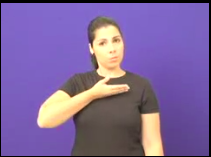
\includegraphics[height=3cm, width=5cm]{src/images/amigo.png}}}%
    \qquad
    \subfloat[Desculpa]{{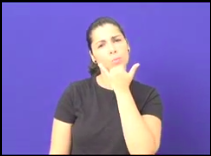
\includegraphics[height=3cm, width=5cm]{src/images/desculpa.png} }}%
    \qquad
    \subfloat[Telefone]{{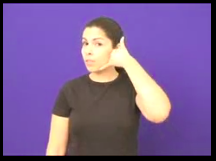
\includegraphics[height=3cm, width=5cm]{src/images/telefone.png} }}%
    \qquad
    \caption{Gestos selecionado para o conjunto de dados}%
    \label{figure:gestos_selecionados}%
    \fonte{Produção do autor} % Adaptado de Dicionário de Libras
\end{figure}

\par Para a aquisição dos dados, foi desenvolvido uma ferramenta (Figura \ref{figure:sistema_aquisicao}) \textit{desktop} multiplataforma na linguagem Python, com o auxílio da biblioteca PyQt, para a criação da interface gráfica e a biblioteca OpenCV, para a manipulação das imagens capturadas.

% Ei!! Problema na imagem, você não declarou ter utilizado o gesto "Idade".... (07/03/2019)
\image{0.60}{recurso_assistivo_escrita_com_gestos/tela_programa_aquisicao_de_dados.png}{Tela inicial da aplicação de aquisição de dados}{figure:sistema_aquisicao}{Produção do Autor}

\par Como apresentado na Figura \ref{figure:sistema_aquisicao}, o sistema de aquisição de imagens demonstra exemplos dos gestos que devem ser reproduzidos pelo usuário, uma barra de progresso, e botões para começar e recomeçar a captura das imagens do usuário e também para saber mais sobre o projeto.

\par Este sistema captura 60 imagens, sendo 20 de cada um dos gestos, em cada uma das imagens capturadas é aplicado uma operação de redimensionamento, isto para que, todas as imagens tenham as dimensões 224x224x3, já que esta é a dimensão aceita pelo \textit{Mobilenet}, o modelo que será retreinado com os dados que estão sendo coletados. Após a aquisição das 60 imagens o programa cria um arquivo no formato zip e o envia para um \textit{email} criado para o armazenamento dos dados.

\par O programa foi distribuído e ao final houveram 11 colabores, criando assim um conjunto com 660 imagens, com quantidades de imagens igualmente distribuídas para cada gesto.

\subsection{Pré-processamento dos dados} 

\par Durante a aquisição das imagens, nenhuma restrição foi emposta aos colaboradores, assim uma etapa de validação de cada uma das imagens teve de ser realizada para garantir que, cada uma das imagens representa o gesto ao qual é indicado, o que resultou na remoção de algumas imagens. A Figura \ref{figure:plot_qtd_apos_filtro} apresenta a relação da quantidade de imagens com cada um dos gestos após a validação realizada.

\image{0.90}{quantidade_de_gestos_por_plot_apos_filtro.jpeg}{Quantidade de imagens por gesto após filtragem}{figure:plot_qtd_apos_filtro}{Produção do Autor}

\par Após esta filtragem, o conjunto de dados foi dividido em treino e teste, ficando 80\% dos dados para treino e 20\% para o teste. Este processo foi criado utilizando a biblioteca sklearn de Python, e o código é apresentado na Figura \ref{figure:split_train_test_data}.

\begin{figure}[H]
    \centering
    \begin{lstlisting}[language=Python]
from sklearn.model_selection import train_test_split

x, y = [], []

for collaborator_dir in os.listdir():
    files = os.listdir(collaborator_dir)

    x.extend(files)
    y.extend(np.repeat(collaborator_dir, len(files)))

x_train, x_test, y_train, y_test = train_test_split(x, y, test_size=0.20, random_state=992)    
\end{lstlisting}
    \caption{\textit{Script} de separação dos dados (Treino X Teste)}
    \fonte{Produção do autor}
    \label{figure:split_train_test_data}
\end{figure}

\par Veja que, para cada colaborador há um diretório contendo as imagens coletadas, estes diretórios são percorridos e cada imagem e o gesto que a mesma representa são salvos em uma lista, que posteriormente é dividida em listas de treino e teste com a função \textitbf{train\_test\_split}.

\par Com a divisão realizada, cada uma das imagens divididas em treino e teste são movidas para os diretórios de seus respectivos tipos. A função criada para esta movimentação é apresentado na Figura \ref{figure:move_splitted_data}.

\begin{figure}[H]
    \centering
    \begin{lstlisting}[language=Python]
def move_data(x_data: list, y_data: list, typeof: str) -> None:
    for xt, yt in zip(x_data, y_data):
        src = os.path.join(yt, xt)
        dst = os.path.join(typeof, yt, xt)
        
        copyfile(src, dst)
\end{lstlisting}
    \caption{Função para movimentação dos arquivos de Treino e Teste}
    \fonte{Produção do autor}
    \label{figure:move_splitted_data}
\end{figure}

\par Com a finalização da separação dos dados, as quantidades de imagens nos conjuntos de treino e teste são apresentados na Figura \ref{figure:qtd_imagem_treino_teste}.

\image{0.80}{quantidade_de_imagem_por_tipo.jpeg}{Quantidade de imagen de treino e teste}{figure:qtd_imagem_treino_teste}{Produção do Autor}

\par Poucas imagens podem ser um problema para a generalização do modelo, mesmo levando em consideração o retreino do \textit{Mobilenet} que será feito, desta forma, por conta disto, será aplicado no conjunto de teste o \textit{Data Augmentation}, que através de modificações nas imagens já existentes cria-se novas imagens, fazendo com que o conjunto de dados aumente.

\par Neste trabalho, o \textit{Data Augmentation} foi realizado com o auxílio do \textit{Augmentor}, uma biblioteca Python que permite a criação de um \textit{Pipeline} de alterações baseado em probabilidade, assim atribui-se para cada alteração que pode ser aplicada na imagem uma probabilidade de ocorrência, e então o \textit{Augmentor} com base nas probabilidades aplica uma ou várias alterações na base de imagens. 

\par A Figura \ref{figure:pipeline_data_augmentation} apresenta todas as alterações que podem ser aplicadas nas imagens durante sua passagem pelo \textit{Pipeline}.

\image{0.90}{recurso_assistivo_escrita_com_gestos/pipeline_de_geracao_de_imagens.jpeg}{Alterações aplicadas no \textit{Pipeline} do \textit{Data Augmentation}}{figure:pipeline_data_augmentation}{Produção do Autor}

\par O trecho de código apresentado na Figura \ref{figure:dataaugmentation} demonstra como é a implementação do \textit{Pipeline} de alterações demonstrados na Figura \ref{figure:pipeline_data_augmentation}.

\begin{figure}[H]
    \centering
    \begin{lstlisting}[language=Python]
import Augmentor

p = Augmentor.Pipeline('gestos_editados/treino')

p.random_distortion(probability=0.5, grid_height=3, grid_width=3, magnitude=2)

p.skew_left_right(probability=0.3, magnitude=0.7)
p.skew_corner(probability=0.4, magnitude=0.5)

p.sample(1500)
    \end{lstlisting}
    \caption{\textit{Script} de \textit{Data Augmentation}}
    \fonte{Produção do autor}
    \label{figure:dataaugmentation}
\end{figure}

\par Veja que, cria-se inicialmente uma instância de \textit{Pipeline} indicando apenas o diretório das imagens de treino, e então todas as possíveis modificações são declaradas na instância de \textit{Pipeline} e junto a cada uma delas uma probabilidade. No fim, é indicado que o total de imagens gerado deve ser 1500.

\par A Figura \ref{figure:gestos_gerados_no_pipeline} apresenta exemplos de imagens geradas com as diferentes modificações indicadas no código.

\begin{figure}[H]%
    \centering
    % \subfloat[]{{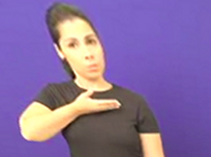
\includegraphics[height=3cm, width=5cm]{src/images/imagens_alteradas_pelo_pipeline/amigo_1.png}}}%
    % \qquad
    \subfloat[]{{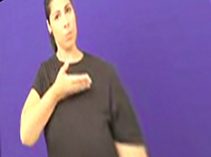
\includegraphics[height=3cm, width=5cm]{src/images/imagens_alteradas_pelo_pipeline/amigo_2.png}}}%
    \qquad
    % \subfloat[]{{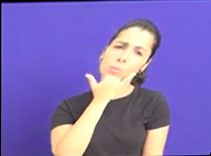
\includegraphics[height=3cm, width=5cm]{src/images/imagens_alteradas_pelo_pipeline/desculpa_1.png}}}%
    % \qquad
    \subfloat[]{{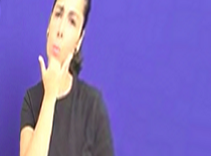
\includegraphics[height=3cm, width=5cm]{src/images/imagens_alteradas_pelo_pipeline/desculpa_2.png}}}%
    \qquad
    \subfloat[]{{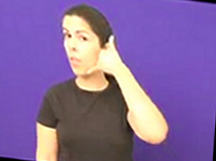
\includegraphics[height=3cm, width=5cm]{src/images/imagens_alteradas_pelo_pipeline/telefone_1.png}}}%
    \qquad
    % \subfloat[]{{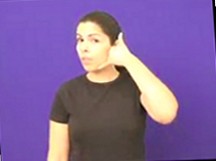
\includegraphics[height=3cm, width=5cm]{src/images/imagens_alteradas_pelo_pipeline/telefone_2.png}}}%
    % \qquad
    \caption{Exemplos de imagens geradas pelo \textit{Pipeline}}%
    \label{figure:gestos_gerados_no_pipeline}
    \fonte{Produção do autor} 
\end{figure}

\par Após a aplicação do \textit{Pipeline} o conjunto de treino passou a ter 1500 imagens, a Figura \ref{figure:plot_qtd_apos_dataaugmentation} mostra este valor distribuído por gesto.

\image{0.90}{imagens_dev/quantidade_de_imagens_por_gesto_apos_da.jpeg}{Quantidade de imagens por gesto com \textit{Data Aumentation}}{figure:plot_qtd_apos_dataaugmentation}{Produção do Autor}

\subsection{Treinamento da Rede Neural Convolucional}

\textbf{ESTA SUBSEÇÃO AINDA SERÁ ESCRITA}

% O modelo de CNN utilizado neste recurso assistivo é criado a partir da aplicação da técnica de aprendizado por transferência no modelo \textit{Mobilenet}.

%%%%% 16/03/2019
% Antes de continuar esta parte será necessário conseguir mais um colaborador, para que então sua imagem seja utilizada no conjunto de testes, para deixar mais coerente os resultados da rede.

% E a camada de convolução inicial foi alterada, desta forma, será utilizado da camada 10 em diante...

% Explicar que a camada 10 foi escolhida já que, quanto mais a frente mais específicos são as características escolhidas pela rede, ou seja, a base é mais genérica (Buscar uma referência)
%%%%%

% \par O modelo treinado é normalmente salvo no formato \textbf{H5}, porém neste caso, ele será convertido para um formato otimizado para \textit{web}, e que poderá ser consumido pelo TFJS.

% Mostrar código da conversão....

\subsection{Distribuição do modelo}

\par Com a finalização do treinamento e conversão do modelo, é necessário criar uma forma que facilite sua distribuição, uma vez que, para a utilização o TFJS carrega o modelo e todos os seus pesos. Neste caso optou-se pela criação de uma \textit{API Rest} para a distribuição do modelo, o que evita aos usuários da biblioteca qualquer necessidade de criar suas próprias formas de distribuição do modelo.

\par A \textit{API Rest} foi criada utilizando Python junto ao Flask. A Figura \ref{figure:exemplo_rota_flask} apresenta o código da rota criada para a distribuição do modelo de reconhecimento de Libras.

% Problemas na formatação da linguagem
\begin{figure}[H]
    \centering
    \begin{lstlisting}[language=Python]
@app.route("/models/mobilenetv1/<file>", methods=["GET"])

@cross_origin()
def mobilenetv1_model(file):
    path = os.path.join(app.config["BASE_DIR"], "api/models/mobilenetv1")

    try:
        return send_from_directory(directory=path, filename=file)
    except:
        return jsonify({
            "error": True,
            "message": "Erro ao tentar recuperar os dados"
        })
    \end{lstlisting}
    \caption{Rota de distribuição do modelo de reconhecimento de Libras}
    \fonte{Produção do autor}
    \label{figure:exemplo_rota_flask}
\end{figure}

\par Para consumir esta \textit{API} e carregar o modelo na biblioteca, criou-se o módulo nomeado \textitbf{MobileNetV1Libras}, que está no conjunto \textitbf{Core} de funcionalidades do ICan.js. O código de consumo da \textit{API} é apresentado na Figura \ref{figure:exemplo_consome_api}.

\begin{figure}[H]
    \centering
    \begin{lstlisting}[language=Javascript]
async buildNet() {
    if (this.model === null) {
        this.model = await tf.loadModel(new URL("/models/mobilenetv1/model.json", MODEL_URL).href);
    }
}
    \end{lstlisting}
    \caption{Método de consumo da \textit{API REST} com o modelo de reconhecimento de Libras}
    \fonte{Produção do autor}
    \label{figure:exemplo_consome_api}
\end{figure}

\subsection{Criação do recurso assistivo}

\par Após todo o processo de treinamento, disponibilização e consumo do modelo de CNN utilizado neste recurso assistivo, foi adicionado no conjunto \textitbf{Common} o componente \textitbf{Writer}, este que permite a escrita em campos de páginas \textit{web} utilizando gestos.

\par Como demonstrado anteriormente, as imagens utilizadas durante o treinamento do modelo são estáticas, porém para garantir a usabilidade, no componente \textitbf{Writer} aplicou-se o método descrito em \cite{Magalh2018}, onde a média de classificações de um conjunto de \textit{frames} capturados em um intervalo de tempo é utilizado para definir qual foi o gesto realizado pelo usuário. Isto permite que, haja mais naturalidade na transformação dos gestos realizados em texto.

\par Toda esta operação é realizado por uma função recursiva, demonstrada na Figura \ref{figure:funcao_recursiva_de_classificacao}, nesta a cada recursão realizada um \textit{frame} é capturado, e quando o número mínimo de \textit{frames} capturados é atingido, tira-se a média das predições e então é feito a definição do gesto a ser escrito. Perceba também que, a recursão da função só é chamada novamente após um intervalo de tempo.

\begin{figure}[H]
    \centering
    \begin{lstlisting}[language=JavaScript]
async function recursiveInterval() {
    try {
        gestures.push(await mobilenetGestures.predictFrame());

        if (gestures.length >= nFrames) {
            fnc(getMeanGesture(gestures));
            gestures = [];
        }

        timeout = window.setTimeout(() => {
            recursiveInterval();
        }, delay * 1000);       
    } catch(err) {
        if (timeout !== null) {
            window.clearTimeout(timeout);
        }

        console.error("librasWriter", err);
    }
}
    \end{lstlisting}
    \caption{\textit{Script} de classificação recursiva}
    \label{figure:funcao_recursiva_de_classificacao}
\end{figure}

\section{Controle de \textit{mouse} com movimentos da cabeça}

\par Este recurso assistivo permite a interação de usuários com deficiência motora a navegação de páginas da \textit{web} com movimentos da cabeça.

% \par O desenvolvimento deste recurso assistivo ocorreu através da utilização do modelo PoseNet junto a regressão linear.

% % Explicação para a avó
% \par Para isto o modelo identifica os pontos do corpo do usuário, os valores da posição do ponto identificado é aplicado em uma regressão, esta que devolve a posição a qual o usuário está  

\subsection{Mapeamento dos movimentos}

\par O mapeamento dos movimentos representa o processo da transformação dos movimentos realizados pelo usuário para movimentos do \textit{mouse}. Neste trabalho utilizou-se os conceitos apresentados em \cite{Papoutsaki2016}, onde os movimentos do usuário são capturados e traduzidos para a tela do computador utilizando regressões.

\par Assim neste trabalho os movimentos dos usuários são capturados utilizando o modelo \textit{PoseNet}, já implementado no TFJS. Com a captura dos movimentos realizadas, a saída da rede é passada para um modelo de regressão, que cria o mapeamento dos movimentos do usuário para a tela do computador. A Figura \ref{figure:flow_mapeamento} apresenta este ciclo completo.

\image{0.80}{recurso_assistivo_controle_do_mouse/flow_de_mapeammento_de_movimentos.jpeg}{Fluxo de funcionamento do mapeamento de movimentos para tela do computador}{figure:flow_mapeamento}{Produção do Autor}

\subsection{Calibração da regressão}

\par Como explicado anteriormente, para o mapeamento dos movimentos do usuário para a tela do computador, é utilizado um modelo de regressão, no caso deste trabalho utilizou-se a regressão linear. 

\par Porém para seu funcionamento é necessário que esta seja ajustada para compreender como realizar a tradução dos resultados do \textit{PoseNet} em posições da tela para movimentação do \textit{mouse}. Este processo é realizado com o auxílio da \textit{API} de calibração presente no módulo \textitbf{Calibration} do conjunto \textitbf{Common}.

\par No módulo \textitbf{Calibration}, são criados 9 pontos na tela do usuário (Figura \ref{figure:tela_de_calibracao_da_regressao}) estes que, ao serem clicados vinculam a posição em que está o nariz do usuário na imagem capturada pela \textit{webcam} com a posição do \textit{mouse}. Desta forma o usuário pode ir mapeamento a posição de seu nariz com a do \textit{mouse}.

\image{0.20}{recurso_assistivo_controle_do_mouse/tela_computador_calibracao_editada.png}{Tela de Calibração}{figure:tela_de_calibracao_da_regressao}{Produção do Autor}

\par O módulo \textitbf{Calibration}, utiliza a biblioteca P5.js para a realização dos desenhos na tela e também o módulo \textitbf{CalibrationAPI} do conjunto \textitbf{Core} do ICan.js que utiliza as capturas realizadas para a calibração da regressão.

\par A função da Figura \ref{figure:funcao_coleta_de_pontos_calibracao} é a responsável pela captura da posição do \textit{mouse} e do nariz do usuário.

\begin{figure}[H]
    \centering
    \begin{lstlisting}[language=JavaScript]
sketch.mousePressed = function() {
    if (poses !== null) {
        let noseObj = {
            x: poses.keypoints[0].position.x,
            y: poses.keypoints[0].position.y
        }
        
        let mouseObj = {
            x: sketch.mouseX,
            y: sketch.mouseY
        }
        calibrationAPI.isInEllipse(mouseObj, noseObj);
    } 
}
    \end{lstlisting}
    \caption{Função de coleta de pontos}
    \label{figure:funcao_coleta_de_pontos_calibracao}
\end{figure}

\par Por padrão, a quantidade de dados coletadas é de 15 amostrar para cada ponto exibido na tela, mas este valor pode ser ajustado. Após esta coleta, os dados são utilizados para a calibração do modelo de regressão no módulo \textitbf{Regression} presente no \textitbf{Core}, assim como é apresentado na função da Figura \ref{figure:funcao_calibracao_modelo_de_regressao}.

\begin{figure}[H]
    \centering
    \begin{lstlisting}[language=JavaScript]
inferMousePosition(nose) {
    if (this.modelX === null || this.modelY === null) {
        throw Error("It is necessary to train the model before using this method");
    }

    let xPredict = (nose.position.x * this.modelX.gradient) + this.modelX.intercept;
    let yPredict = (nose.position.y * this.modelY.gradient) + this.modelY.intercept;

    if (this.filter !== null) {
        if (this.stack.x.length === this.filter.delay) {
            xPredict = this.filter.apply(this.stack.x);
            yPredict = this.filter.apply(this.stack.y);

            this.stack = { x: [], y: [] };
        } else {
            this.stack.x.push(xPredict);
            this.stack.y.push(yPredict);
        }
    }
    return {
        x: xPredict,
        y: yPredict
    }
}
    \end{lstlisting}
    \caption{Função de calibração do modelo}
    \label{figure:funcao_calibracao_modelo_de_regressao}
\end{figure}

\par Veja na Figura \ref{figure:funcao_calibracao_modelo_de_regressao} que, com os dados inseridos dois modelos de regressão são treinados, estes representando primeiramente a posição X do \textit{mouse} e do nariz do usuário e a posição Y dos mesmos.

\subsection{Criação do recurso assistivo}

\par Com a definição do método de mapeamento dos movimentos da cabeça do usuário o recurso assistivo pode ser desenvolvido. Assim, foi adicionado o componente \textitbf{Viewer} no conjunto de funcionalidades \textitbf{Common} do ICan.js, desta forma o usuário passa a conseguir navegar pelas páginas da \textit{web} utilizando movimentos da cabeça.

\par Veja que, o que o módulo \textitbf{Viewer} faz é basicamente criar uma forma de alto nível de unificar o modelo de regressão já treinado com as saídas do \textit{PoseNet}.
